\chapter{Implementation}
\label{chapter:implementation}

\section{Eos}
In order to build anything related to EVE fits, an engine is needed that can parse raw Dogma and spit out ship and item attributes. This is where Eos comes in, an engine developed by the community behind pyfa \cite{pyfa}, a popular fitting tool.

The first thing Eos has to do is read the inventory and dogma tables through an abstraction layer that lets you define data handlers which will read these tables. After that, Eos cleans the tables of unnecessary data and performs some transformations on them (hardcoding some missing attributes, moving some rows between tables. etc) and builds a cache which it then stores on disk. Future work will involve making an abstraction layer for cache handling so that users can put in their own handlers to store the cache how they see fit.

The main functionality of Eos is exposed through the Fit class. This class encapsulates the restriction tracker which is used to validate the fit. Some items can impose certain restrictions like not having more than one module of the same kind active at the same time, while others can only be fitted on specific groups of ships. Almost all modules have skill restrictions, which specify that the character must have the appropriate skills trained to a certain level in order to use that module. All these rules are verified by the restriction tracker which will raise validation errors in case any of them is not respected.

The Fit class encapsulates the module racks which are lists of abstract holders that can contain items, along with their attributes and effects. Each attribute has a list of modules that affect it, so tracking who affects what is fairly easy and efficient. When calculating the final value of an attribute, one must take into account the stacking penalty \cite{stacking}, which specifies that if more than one module that affects the same attribute are fitted on a fit, then their efficiency will suffer. This means that a single module will apply 100\% of its effect to an attribute, while the second one will have a slightly lower weight in the final result. When calculating the penalties for modules, they are first sorted by the value of their bonus. Modules that apply a higher bonus will do so with a higher efficiency that modules affecting the same attribute, but with a smaller bonus. Iterating through this list, the stacking penalty is calculated using an exponential based on the module’s position in the list. The 12th module and further are ignored, since, after the stacking penalty is applied, their influence on the final result is negligible. To make the calculations faster, a lookup table is used that stores the stacking penalties for up to 12 modules.

After the final values are calculated, they are cached and are only recalculated when the list of affectors is changed, by adding or removing modules. This makes for very efficient updates of the underlying fit, due to only the attributes that are affected by the update being recalculated.

\section{Raven}
Handling raw Dogma is only part of the solution. In order to build a proper fitting tool, one must go a level higher than pure Dogma.

Raven is a high-level library built on top of Eos that’s designed to output more meaningful information about ships. To do this, it inherits from the Fit class declared in Eos and it adds a number of useful methods. By doing so, it provides transparency as users can still access the class as they normally would  in Eos, but with the added benefit of those new methods.

The difficulty when it comes to using Eos directly is that you have to query the ship’s attributes by their ids, which not only makes it difficult, but it can lead to inconsistencies as those ids could change at some point. Raven solves this by providing named properties for the most common attributes.

Most of these properties are just for convenience purposes as they only return the value of a single attribute. Some of them, however, convert and calculate these attributes to provide the final output. For instance, duration attributes are expressed in Dogma using milliseconds as a unit. Raven converts these attributes to seconds, as that is the unit used by players. Users can still get the original attribute by querying Eos directly.

Another use case that Raven simplifies is querying for the ship’s shields, armor or hull. Using Eos would require many attribute lookups, but Raven returns a dictionary with all the information one could want.

Another feature, and probably the most important one, is the drain simulator used to simulate capacitor and shield usage. As mentioned in the research chapter, the ship’s capacitor and shields share the same non-linear recharge function. This makes it difficult for players to estimate their cap usage and damage sustainability. Raven implements a simulator which takes into account the effects of all the modules on the ship that affect the capacitor or shields and finds the point or points where the capacitor/shields can sustain the drain. If no such point or points exist, then it calculates the time until the capacitor or shields fully deplete.

The simulator doesn’t differentiate between shields or capacitor. Instead, it takes a number of arguments that define the resource (shields or capacitor) being simulated and a list of arguments defining the modules that affect that resource.

For the resource being simulated, it only needs to know its capacity and recharge time. As for the modules, it needs to know the activation cost and cycle time for each of them.

A naive solution would be to just divide the resource’s capacity by its recharge time, thus obtaining a linear recharge rate. If this rate is higher than the sum of all linear drain rates of the modules, then the resource is stable, otherwise it will fully deplete.

The problem with that solution is that it assumes a linear recharge rate. Thus, if the capacitor can sustain the modules, it will be stable at 100%. That is never the case in real life.

Another approach would be to assume that the modules have drain over time, rather than instantaneous. Coupled with the real formula for recharge rate described in the research chapter, this approach would lead to close approximations of the stability points. Not only that, but it would also be very computationally light, requiring only to solve an equation. 

The most accurate solution would involve treating the module’s activation cost as an instantaneous drain. This would result in a discontinuous drain function that cannot be intersected with the recharge function. Thus, Raven would have to apply both functions step by step and calculate the stability points, if they exist. However, this would require a lot of compute time since the simulator has to run until the capacitor stabilizes.

\section{Tengu}
While a fitting engine is useful in its own right, a GUI must be made to leverage its power. Our main objectives with the UI were to provide an elegant interface that is similar to the one used in EVE Online, all the while providing a user experience that attracts all the types of players.

The first step in building the UI was the layout, which had to be functional and elastic\footnote{A web page with an elastic layout will adapt to the browser’s window dimensions and font preferences.}. We decided on a three column setup with a footer and a header. While the middle column is used to display the main content, the first and third column are used as sidebars and contain various additional information.

There are a few ways to make this kind of layout elastic, including using percentages and em’s \cite{em}. However, when padding, margins and borders are involved, this no longer works\footnote{Specifying the dimensions of an element only affects the inner content and doesn’t take into account any padding, margins or borders.}. Thus, we resorted to using Javascript to automatically adjust the layout when the window resizes. On page load, the width of the main column is calculated as the difference between the window width and the widths of the two sidebars, which are fixed. When the window resizes, so does the content, while every column is set to stretch to occupy the entire available height.

We tried to follow some semantical guidelines when writing markup so as to support various screen readers and web scrapers. Extra markup, such as containers, was only used when absolutely necessary, like for positioning elements inside the layout. We foresee some rewriting in the future to make the markup even more semantically correct.

\subsection{Market browser}
After the layout has been designed, we moved on to create the market browser, which would reside in the left sidebar. The upper part would house the browser, while the lower part would accommodate the list of items in the currently selected group. These two parts are separated by a handler which can be used to resize them. At the very top of the left sidebar resides a search box, which is tab-aware, and is used to search through items and fits. The position of the handler (and, thus, the heights of both parts) is persisted through a cookie.

\begin{figure}[h]
\centering
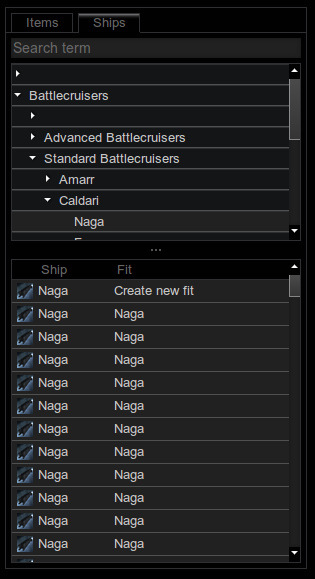
\includegraphics[scale=0.5]{src/img/marketbrowser}
\caption{The market browser}
\label{fig:marketbrowser}
\end{figure}

The market browser has two tabs, one for ships and one for any item that can be fitted to a ship. Both would display a hierarchical view of the market groups available in the game, each treating differently the leaf groups. When clicking on a leaf group in the items tab, the list in the bottom part of the sidebar would load the items available in that group. However, in the ships tab, the leaf groups are the items themselves, which are actually ships. Clicking on one of them would fetch the list of fits for that ship.

Because the items are static, they are cached on the client side using a dictionary so that future requests on the same market group will not result in a new query being sent to the server. Furthermore, the entire market browser is cached on the server side using memcached \cite{memcached} so as to make the page load extremely fast.

The market browser implements a few user experience features designed to make the life of the user easier. Firstly, when a user clicks on a market group, the height of which is larger than the height of the container, the container is automatically scrolled to the top of the market group. This allows to fit as much content of that market group as possible while still retaining its name at the very top. Secondly, when a market group is collapsed, all child groups are collapsed as well. In lack of this feature, expanding that group again would present the user with a mess of previously opened groups. Moreover, the list of collapsed market groups is persisted between sessions through a cookie so as to present the user with the same, consistent browser state.

\subsection{Fitting wheel}
The fitting wheel was a lot of work. It is a custom design based on the one available in EVE and it’s made completely out of vector shapes, so, if the future requires it, it can be resized without any loss of quality. The wheel is transparent to allow the picture of the ship to be seen beneath it and so as to not require any modifications when the background changes.

\begin{figure}[h]
\centering
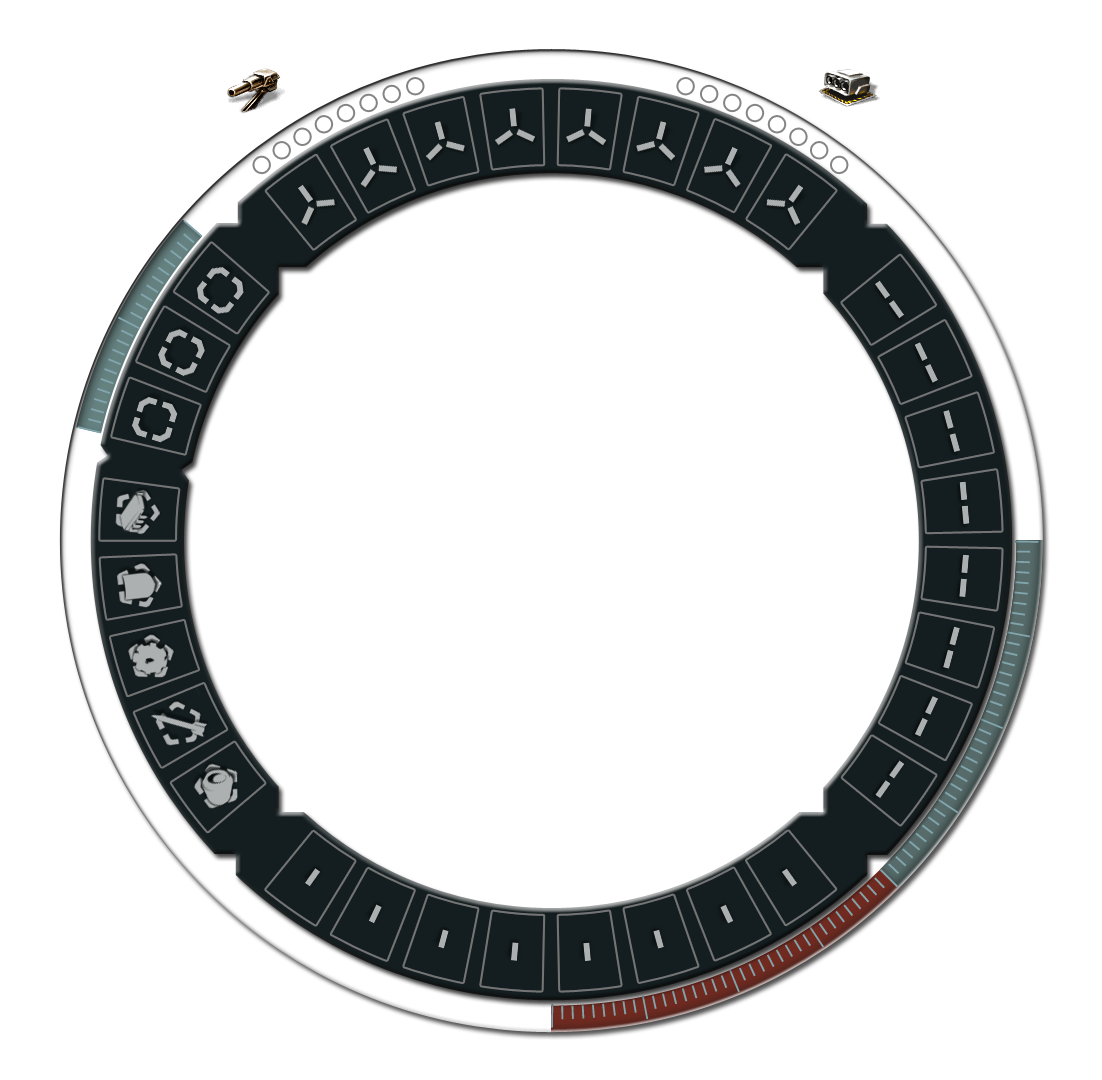
\includegraphics[width=0.7\linewidth]{src/img/wheel}
\caption{The fitting wheel on a transparent background.}
\label{fig:wheel}
\end{figure}

When a ship is loaded, the number of slots are retrieved from the database and the template associates each rack a CSS class that will load the proper icons. There are 8 icon sets available for each rack in the form of rack\_nrslots.png which represents the appropriate number of slots in that specific rack. These are absolutely positioned so as to align perfectly with the rest of the wheel. The initial design would involve styling each slot separately through absolute positioning and CSS3 transformations, but this would have required extra markup and could have caused compatibility issues between browsers (especially the ingame one).

Each slot was manually aligned to make them all equally spaced, while everything was aligned using guides, resulting in a pixel perfect arrangement. The scale units are actually pipes (“|”) typed on a circular path and carefully stretched and aligned to fill the required space. The larger units were individually adjusted to be equally spaced and wide like the rest.

Handling the placement of module icons on the wheel was no easy task. We set out to implement each rack as a sortable list using the jQuery UI Sortable widget. But we soon found out it doesn’t support elements that are absolutely positioned, a feature we required in order to align each module with its corresponding slot. We solved this by creating a list of divs that have equal height, but each contain variably padded handles that will contain the actual module icon. The Sortable widget was set to only drag elements by their handles, which would give the appearance of individually positioned elements. Each element was styled according to its position in the list using the nth-type-of CSS3 selector \cite{nthtypeof}.

However, we hit another roadblock. When an element from the list is picked up, the Sortable widget creates a placeholder element which is used to indicate the spot where the element will be dropped. This element is appended after the original element, thus, shifting the indices of all the other elements after it by 1. This was breaking the CSS selectors as they were now counting the placeholder as well. After much tinkering with the Sortable API \cite{sortable}, we attached callbacks to the start and stop events that are triggered when sorting starts and, respectively, stops, that take the element being dragged and move it to the end of the list, leaving the placeholder in its original place. Doing so won’t break any selectors as the elements are still in their original slots. When the sorting stops, the original element is placed instead of the placeholder, which is removed by the widget.

This is an innovative approach to this problem and we plan to release a separate, open-source plugin that will create a circular sortable list using the Sortable widget and the tricks outlined above. We hope that it will help many other people in need of such a plugin.

\section{Stats widgets}

\begin{figure}[h]
\centering
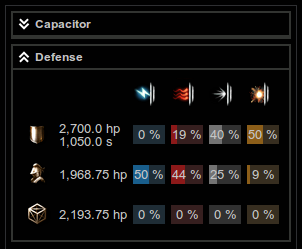
\includegraphics[scale=0.5]{src/img/stats}
\caption{Example of a stats widget}
\label{fig:stats}
\end{figure}

After the market browser and fitting wheel were working properly, we moved on to style the widgets responsible with displaying the various statistics. These were made to resemble as closely as possible the ones present in the game, so as to provide a pleasant and familiar experience to the users.

The widgets are individually collapsable and their state is persisted between sessions through cookies. We went a step further and made their state synchronized between all open tabs. That means that every time a user changes the order of the widgets or collapses or expands one of them, every instance of them is synchronized. This provides a sense of consistency and a level of customization rarely seen in web apps.


\section{Tabs}

In order to support viewing multiple fits at the same time, we had to implement support for tabs. A proper framework was written which supports sortable tabs that can be linked with multiple content panes that will be shown when the linked tab gains focus. These panes can be linked through ids or even directly by object, for scenarios where ids can’t be assigned yet (e.g. when content is being loaded).

\begin{figure}[h]
\centering

\includegraphics[width=0.7\linewidth]{src/img/tabs}
\caption{Multiple opened fit tabs}
\label{fig:tabs}
\end{figure}

When a tab is closed, the framework automatically places the focus on the rightmost tab, if one exists. Closing tabs also triggers events that can be caught by other scripts which can register callbacks to perform various custom actions. One particular example is when closing the last fit tab, in which case a welcome tab is displayed that instructs the user to use the market browser to create a new fit or edit an existing one. When a new tab is opened, the welcome tab is hidden, only to be revealed again when the last one is closed.

\section{Service layer}
As an integrated part of Tengu, the service layer handles storing and accessing fits from the database, as well as user management and authentication.

\begin{figure}[h]
\centering
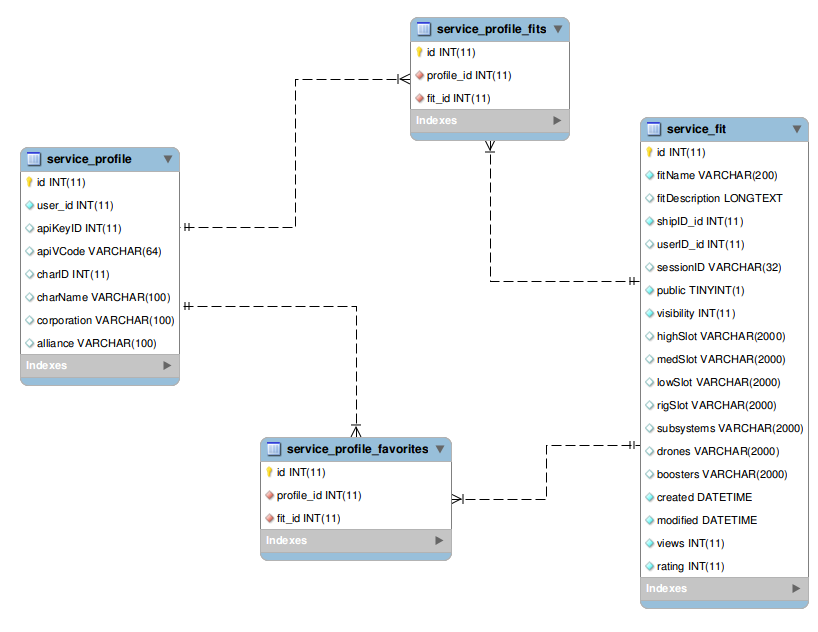
\includegraphics[width=0.7\linewidth]{src/img/service}
\caption{Service tables}
\label{fig:service}
\end{figure}

Every user has an associated profile, which, among various additional information that are not present in the standard Django user model, stores an API key which is used to retrieve information about the ingame character from the Tranquility server. This information includes the character name, which is displayed next to a fitting so that EVE players can easily recognize the author. Moreover, the character’s corporation and alliance names are fetched to allow saving fits that will be made visible to the entire corporation or alliance.

Permission checking is performed before fetching the fits so as to not let users view private fits, or fits belonging to a different corporation or alliance. Because Django’s filter() method \cite{filter} only supports simple queries with “ANDed” arguments, we use Q objects \cite{q} to perform more complex searches. Q objects can be combined using the \& and | operators, resulting in a new Q object.

\begin{lstlisting}[caption=An example of using Q objects, language=python]
if request.user.pk:
  return Q(userID = request.user.pk) | Q(public=True)

return Q(sessionID = request.session.session_key) | Q(public=True)
\end{lstlisting}

Requesting the corporation and alliance name from the EVE API servers every time a permission check is performed would make queries take a very long time to complete. To solve this issue, we only query the API once per day, for all the users, and store the needed information in our database. That way, a search query would need not interrogate the API servers, as the information would already be available offline. A cron job is setup to handle fetching and updating the information for all the users.

The service layer also exposes an API that 3rd party developers can use to interact with Tengu. The API provides calls for retrieving fittings in various formats, which can include JSON, HTML and text-only. 